\documentclass[12pt,a4paper]{article}
\usepackage[utf8]{inputenc}
\usepackage[turkish]{babel}
\usepackage{amsmath,amssymb,amsfonts,amsthm}
\usepackage{geometry}
\geometry{top=2.5cm,bottom=2.5cm,left=2.5cm,right=2.5cm}
\usepackage{xcolor}
\usepackage{tikz}
\usetikzlibrary{babel,arrows.meta,positioning,calc}
\usepackage{pgfplots}
\pgfplotsset{compat=1.18}
\usepackage[most]{tcolorbox}
\usepackage{hyperref}
\usepackage{caption}
\usepackage{booktabs}
\usepackage{tabularx}

% -------------------------------------------------
% style.tex – Ortak paketler ve tcolorbox tanımları
% -------------------------------------------------
\usepackage[utf8]{inputenc}
\usepackage[turkish]{babel}
\usepackage{amsmath,amssymb,amsfonts,amsthm}
\usepackage{geometry}
\geometry{top=2.5cm,bottom=2.5cm,left=2.5cm,right=2.5cm}
\usepackage{xcolor}
\usepackage{tikz,pgfplots}
\pgfplotsset{compat=1.18}
\usepackage[most]{tcolorbox}
\usepackage{hyperref}
\usepackage{caption,booktabs,tabularx}

% ---------- Renk tanımları ----------
\definecolor{purp}{RGB}{102,51,153}
\definecolor{tealblue}{RGB}{0,120,130}
\definecolor{mainblue}{RGB}{26,82,118}
\definecolor{alertred}{RGB}{180,40,40}
\definecolor{okgreen}{RGB}{34,139,34}

% ---------- Tek‑argümanlı kutular ----------
\newtcolorbox{box}[2][]{
  colback=white,
  colframe=purp,
  title={#2},
  arc=2mm,
  breakable,
  #1
}

\newtcolorbox{uyari}[1][]{
  colback=yellow!10,
  colframe=orange,
  title={Uyarı},
  arc=2mm,
  breakable,
  #1
}

% ---------- Diğer yardımcı kutular (isteğe bağlı) ----------
\newtcolorbox{ornek}[2][]{
  colback=mainblue!5!white,
  colframe=mainblue,
  title={#2},
  arc=2mm,
  breakable,
  #1
}

\newtcolorbox{odev}[2][]{
  colback=okgreen!5!white,
  colframe=okgreen,
  title={Çözümü Olmayan Ödev ve Tam Çözümü: #2},
  arc=2mm,
  breakable,
  #1
}

\newtcolorbox{tanim}[2][]{
  colback=gray!5!white,
  colframe=gray!60!black,
  title={#2},
  arc=2mm,
  breakable,
  #1
}

\newtcolorbox{sezgi}[2][]{
  colback=tealblue!5!white,
  colframe=tealblue,
  title={Sezgisel Bakış ve Basit Anlatım: #2},
  arc=2mm,
  breakable,
  #1
}

\title{\textbf{İSTATİSTİK TEORİSİ}\\[0.3em] \Large 3. Hafta Ders Notları ve Detaylı Konu Anlatımı}
\author{Ders Notları Düzenlemesi, Sezgisel Açıklamalar ve Çözümlü Analizler}
\date{}

\begin{document}
\maketitle

\begin{abstract}
Bu çalışma; İstatistik Teorisi dersinin 3. haftasında yer alan \textbf{Yakınsama Türleri} (Olasılıkta, Hemen Hemen Her Yerde, Momentte ve Dağılımda), \textbf{Merkezi Limit Teoremi (CLT / MLT)}, \textbf{Slutsky Teoremi}, \textbf{Sıra İstatistiklerinin Limitleri} ve \textbf{Ki-Kare Dağılımının Normale Yakınsaması} konularını içermektedir. Ağır matematiksel teoremler sezgisel benzetmeler ve çözümlü örneklerle basitleştirilmiştir.
\end{abstract}

\hrule
\vspace{1em}

\section{Büyük Resim: Örneklem Büyüdükçe (\texorpdfstring{$n \to \infty$}{n sonsuza giderken}) Ne Olur?}

Lisede veya kalkülüste bir sayı dizisinin limitini biliriz: Örneğin $a_n = \frac{1}{n} \to 0$. Sayılar sabittir ve nereye gittikleri bellidir.  
Ancak istatistikte elimizde sayılar değil, **rastgele değişkenler** ($X_1, X_2, \dots, X_n$) vardır!  
Her denemede farklı bir sonuç üreten bir sürecin "limiti" ne demektir?
\begin{itemize}
    \item Değişkenin kendisi tek bir sabit sayıya mı yaklaşır? $\longrightarrow$ \textbf{Olasılıkta Yakınsama} ($X_n \xrightarrow{P} c$)
    \item Her bir deneme kesinlikle aynı hedefe mi varır? $\longrightarrow$ \textbf{Hemen Hemen Her Yerde Yakınsama} ($X_n \xrightarrow{a.s.} X$)
    \item Değişkenin kendisi sabit kalmasa bile, çizdiği olasılık eğrisi (grafiği) tanıdık bir şekle mi bürünür? $\longrightarrow$ \textbf{Dağılımda Yakınsama} ($X_n \xrightarrow{d} X$)
\end{itemize}

---

\section{Rastgele Değişken Dizilerinde Yakınsama Türleri}

\subsection{1. Olasılıkta Yakınsama (Convergence in Probability)}

\begin{sezgi}{Olasılıkta Yakınsamanın Anlamı: Hedefte Toplanma}
Bir hedef tahtasına sürekli ok attığınızı hayal edin ($n$ ok sayısı). $n$ büyüdükçe merkezin $\epsilon$ kadar uzağına düşme ihtimaliniz sıfıra iniyorsa, yani atışlarınızın \%99.999'u hedefin minicik bir çevresine sıkışıyorsa bu dizi hedefe **olasılıkta yakınsıyor** demektir.
\end{sezgi}

\begin{tanim}{Olasılıkta Yakınsama ($X_n \xrightarrow{P} X$)}
Her $\epsilon > 0$ için:
\begin{equation}
    \lim_{n \to \infty} P\left( |X_n - X| \ge \epsilon \right) = 0 \quad \iff \quad \lim_{n \to \infty} P\left( |X_n - X| < \epsilon \right) = 1
\end{equation}
ise $X_n$ dizisi $X$'e \textbf{olasılıkta yakınsar} denir ve $X_n \xrightarrow{P} X$ ile gösterilir.
\end{tanim}

\begin{ornek}{Örnek 1: Zayıf Büyük Sayılar Yasası (WLLN)}
$X_1, \dots, X_n \overset{\text{i.i.d.}}{\sim} (\mu, \sigma^2 < \infty)$ olsun. Örneklem ortalaması $\bar{X}_n = \frac{1}{n} \sum_{i=1}^n X_i$'nin kitle ortalamasına olasılıkta yakınsadığını ($\bar{X}_n \xrightarrow{P} \mu$) gösteriniz.

\bigskip
\textbf{Çözüm (Chebyshev Eşitsizliği İle):}
Örneklem ortalamasının beklenen değeri ve varyansı:
\begin{equation}
    E(\bar{X}_n) = \mu, \quad V(\bar{X}_n) = \frac{\sigma^2}{n}
\end{equation}
Chebyshev eşitsizliğini uygulayalım:
\begin{equation}
    P\left( |\bar{X}_n - \mu| \ge \epsilon \right) \le \frac{V(\bar{X}_n)}{\epsilon^2} = \frac{\sigma^2}{n \epsilon^2}
\end{equation}
$n \to \infty$ iken limit alırsak:
\begin{equation}
    0 \le \lim_{n \to \infty} P\left( |\bar{X}_n - \mu| \ge \epsilon \right) \le \lim_{n \to \infty} \frac{\sigma^2}{n \epsilon^2} = 0
\end{equation}
Sandviç kuralından olasılık sıfıra gider. Böylece:
\begin{equation}
    \boxed{\bar{X}_n \xrightarrow{P} \mu}
\end{equation}
\textit{Sezgisel Anlamı:} Madeni parayı 10 kez atarsanız \%70 yazı gelebilir. Ama 10.000 kez atarsanız yazı oranı kesinlikle 0.50'ye kilitlenir!
\end{ornek}

\begin{ornek}{Örnek 2: Örneklem Varyansının Tutarlılığı ($S_n^2 \xrightarrow{P} \sigma^2$)}
Normal kitlede örneklem varyansı $S_n^2$'nin kitle varyansı $\sigma^2$'ye olasılıkta yakınsadığını gösteriniz.

\bigskip
\textbf{Çözüm:}
Normal dağılımda $\frac{(n-1)S_n^2}{\sigma^2} \sim \chi^2_{n-1}$ olduğundan varyansı:
\begin{equation}
    V(S_n^2) = \frac{\sigma^4}{(n-1)^2} \cdot 2(n-1) = \frac{2\sigma^4}{n-1}
\end{equation}
Chebyshev eşitsizliğinin tümleyenini yazalım:
\begin{equation}
    P\left( |S_n^2 - \sigma^2| < \epsilon \right) \ge 1 - \frac{V(S_n^2)}{\epsilon^2} = 1 - \frac{2\sigma^4}{(n-1)\epsilon^2}
\end{equation}
$n \to \infty$ iken limit 1 olur. Dolayısıyla $S_n^2 \xrightarrow{P} \sigma^2$'dir; yani $S_n^2$ \textbf{tutarlı (consistent)} bir tahmin edicidir.
\end{ornek}

\subsection{2. Kesinlikle / Hemen Hemen Her Yerde Yakınsama (Almost Sure)}

\begin{tanim}{Kesinlikle Yakınsama ($X_n \xrightarrow{a.s.} X$)}
Örneklem uzayındaki istisnai olayların olasılığı sıfır olmak üzere, sürecin kendisi $X$'e yakınsıyorsa:
\begin{equation}
    P\left( \lim_{n \to \infty} X_n = X \right) = 1
\end{equation}
ise $X_n \xrightarrow{a.s.} X$ denir. (Bu, olasılıkta yakınsamadan çok daha güçlü bir yakınsamadır: $X_n \xrightarrow{a.s.} X \implies X_n \xrightarrow{P} X$).
\end{tanim}

\subsection{3. Momentlerde Yakınsama (\texorpdfstring{$L^r$ Yakınsama}{Lr Yakınsama})}

\begin{tanim}{Momentlerde Yakınsama ($X_n \xrightarrow{L^r} X$)}
$r > 0$ pozitif bir tam sayı olmak üzere:
\begin{equation}
    \lim_{n \to \infty} E\left( |X_n - X|^r \right) = 0
\end{equation}
ise $X_n \xrightarrow{L^r} X$ denir. Özellikle $r=2$ durumuna \textbf{Ortalama Karede Yakınsama (Mean Square Convergence)} adı verilir.
\end{tanim}

\begin{ornek}{Örnek 3: Olasılıkta Yakınsayıp Momentte Yakınsamayan Meşhur Dizi}
$X_n$ rastgele değişkeni şu olasılıklarla tanımlansın:
\begin{equation}
    P(X_n = n^3) = \frac{1}{n^2}, \quad P(X_n = 0) = 1 - \frac{1}{n^2}
\end{equation}
Bu dizinin $X=0$'a yakınsaklığını inceleyiniz.

\bigskip
\textbf{Çözüm:}
\begin{enumerate}
    \item \textbf{Olasılıkta Yakınsama:}  
    Herhangi bir $\epsilon > 0$ için $n$ büyüdüğünde $n^3 > \epsilon$ olur:
    \begin{equation}
        P(|X_n - 0| \ge \epsilon) = P(X_n = n^3) = \frac{1}{n^2} \xrightarrow{n \to \infty} 0
    \end{equation}
    Demek ki \textbf{olasılıkta sıfıra yakınsar} ($X_n \xrightarrow{P} 0$).
    \item \textbf{1. Momentte ($r=1$) Yakınsama:}
    \begin{equation}
        E(|X_n - 0|) = E(X_n) = n^3 \cdot \left(\frac{1}{n^2}\right) + 0 \cdot \left(1 - \frac{1}{n^2}\right) = n \xrightarrow{n \to \infty} \infty \neq 0
    \end{equation}
    Ortalaması sonsuza patladığı için \textbf{momentte yakınsamaz}!
\end{enumerate}
\textit{Püf Noktası:} Nadir görülen devasa uç değerler (black swan) olasılığı sıfıra çekse de ortalamayı havaya uçurabilir!
\end{ornek}

\subsection{4. Dağılımda Yakınsama (Convergence in Distribution)}

\begin{tanim}{Dağılımda Yakınsama ($X_n \xrightarrow{d} X$)}
$X_n$'nin birikimli dağılım fonksiyonu $F_n(x)$ olsun. $F(x)$'in sürekli olduğu her noktada:
\begin{equation}
    \lim_{n \to \infty} F_n(x) = F(x) \quad \iff \quad \lim_{n \to \infty} M_{X_n}(t) = M_X(t)
\end{equation}
ise $X_n \xrightarrow{d} X$ denir.
\end{tanim}

\begin{center}
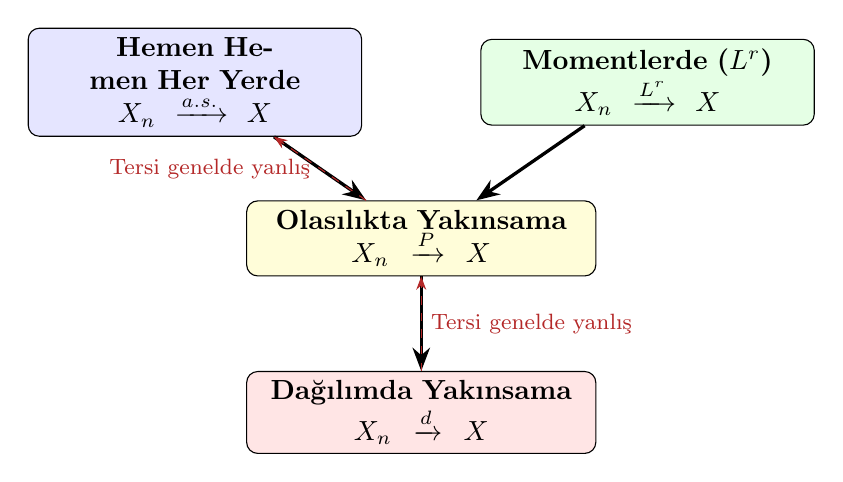
\begin{tikzpicture}[node distance=1.8cm, auto, >=Stealth]
    \node[draw, rounded corners, fill=blue!10, text width=4cm, align=center] (as) {\textbf{Hemen Hemen Her Yerde}\\$X_n \xrightarrow{a.s.} X$};
    \node[draw, rounded corners, fill=green!10, text width=4cm, align=center, right=1.5cm of as] (rm) {\textbf{Momentlerde ($L^r$)}\\$X_n \xrightarrow{L^r} X$};
    \node[draw, rounded corners, fill=yellow!15, text width=4.2cm, align=center, below=1.5cm of $(as)!0.5!(rm)$] (prob) {\textbf{Olasılıkta Yakınsama}\\$X_n \xrightarrow{P} X$};
    \node[draw, rounded corners, fill=red!10, text width=4.2cm, align=center, below=1.2cm of prob] (dist) {\textbf{Dağılımda Yakınsama}\\$X_n \xrightarrow{d} X$};

    \draw[->, very thick] (as) -- (prob);
    \draw[->, very thick] (rm) -- (prob);
    \draw[->, very thick] (prob) -- (dist);
    \draw[->, dashed, alertred] (prob) -- node[left, font=\footnotesize]{Tersi genelde yanlış} (as);
    \draw[->, dashed, alertred] (dist) -- node[right, font=\footnotesize]{Tersi genelde yanlış} (prob);
\end{tikzpicture}
\captionof{figure}{Yakınsama türleri arasındaki hiyerarşik ilişki. Dağılımda yakınsama en zayıf olanıdır.}
\end{center}

\vspace{0.5em}
\section{Merkezi Limit Teoremi (CLT / MLT) ve İspatı}

\begin{sezgi}{İstatistiğin En Büyük Mucizesi: CLT}
Evrendeki ana kitle ister çarpık, ister iki tepeli, isterse tamamen düzensiz olsun; o kitleden bağımsız yeterince büyük ($n \ge 30$) örneklemler çekip ortalamalarını aldığınızda, bu ortalamaların grafiği **kusursuz bir Çan Eğrisi (Normal Dağılım)** oluşturur!
\end{sezgi}

\begin{tanim}{Merkezi Limit Teoremi (Central Limit Theorem)}
$X_1, X_2, \dots, X_n$ bağımsız ve özdeş dağılımlı ($E(X_i)=\mu, V(X_i)=\sigma^2 < \infty$) değişkenler olsun. Standardize edilmiş değişken $n \to \infty$ iken:
\begin{equation}
    Z_n = \frac{\bar{X}_n - \mu}{\sigma / \sqrt{n}} = \frac{\sum_{i=1}^n (X_i - \mu)}{\sigma \sqrt{n}} \xrightarrow{d} N(0, 1)
\end{equation}
\end{tanim}

\subsection{CLT'nin MÇF İle Adım Adım İspatı}
\begin{enumerate}
    \item $Z_n = \sum_{i=1}^n \frac{X_i - \mu}{\sigma\sqrt{n}}$ değişkeninin MÇF'sini yazalım:
    \begin{equation}
        M_{Z_n}(t) = \left[ M_{X - \mu}\left( \frac{t}{\sigma\sqrt{n}} \right) \right]^n
    \end{equation}
    \item $M_{X-\mu}(s)$ fonksiyonunu $s=0$ etrafında Taylor serisine açalım:
    \begin{equation}
        M_{X-\mu}(s) = 1 + s \underbrace{E(X - \mu)}_{0} + \frac{s^2}{2} \underbrace{E[(X - \mu)^2]}_{\sigma^2} + o(s^2) = 1 + \frac{\sigma^2 s^2}{2} + o(s^2)
    \end{equation}
    \item Burada $s = \frac{t}{\sigma\sqrt{n}}$ yazarsak:
    \begin{equation}
        M_{X-\mu}\left( \frac{t}{\sigma\sqrt{n}} \right) = 1 + \frac{\sigma^2}{2} \frac{t^2}{\sigma^2 n} + o(1/n) = 1 + \frac{t^2/2}{n} + o(1/n)
    \end{equation}
    \item Analizdeki meşhur $\lim_{n \to \infty} (1 + \frac{a}{n})^n = e^a$ limit kuralını uygulayalım ($a = t^2/2$):
    \begin{equation}
        \lim_{n \to \infty} M_{Z_n}(t) = \lim_{n \to \infty} \left( 1 + \frac{t^2/2}{n} \right)^n = \boxed{\exp\left( \frac{t^2}{2} \right)}
    \end{equation}
    \item $e^{t^2/2}$ fonksiyonu Standart Normal Dağılım $N(0, 1)$'in MÇF'si olduğundan teklik ve süreklilik teoreminden:
    \begin{equation}
        Z_n \xrightarrow{d} N(0, 1)
    \end{equation}
\end{enumerate}

\vspace{0.5em}
\section{Slutsky Teoremi ve Sıra İstatistiklerinin Limitleri}

\begin{tanim}{Slutsky Teoremi}
$X_n \xrightarrow{d} X$ (dağılımda yakınsayan) ve $Y_n \xrightarrow{P} c$ (bir sabite olasılıkta yakınsayan) ise:
\begin{enumerate}
    \item $X_n + Y_n \xrightarrow{d} X + c$
    \item $X_n Y_n \xrightarrow{d} c X$
    \item $\frac{X_n}{Y_n} \xrightarrow{d} \frac{X}{c} \quad (c \neq 0)$
\end{enumerate}
\end{tanim}

\begin{uyari}
\textbf{Sıra İstatistiği Tanımındaki Not Hatası (Sayfa 17):}
Notlarda $X_i \sim \text{Uniform}(0, 1)$ bağımsız değişkenleri için hem $Y_n$ hem de $Z_n$ minimum olarak yazılmıştır:
\begin{equation*}
    Z_n = \min(X_1, \dots, X_n) \quad \text{\textbf{\textcolor{red}{(NOTTAKİ YAZIM HATASI)}}}
\end{equation*}
ve ardından $Z_n \xrightarrow{P} 1$ gösterilmiştir.  
Doğrusu $Z_n = \mathbf{\max(X_1, \dots, X_n)}$ olmalıdır; nitekim kullanılan $f_{Z_n}(z) = n z^{n-1}$ yoğunluğu maksimum sıra istatistiğine aittir.
\end{uyari}

\begin{ornek}{Örnek 4: Uniform(0,1) Uç Değerlerinin Yakınsaması}
$X_1, \dots, X_n \overset{\text{i.i.d.}}{\sim} \text{Uniform}(0, 1)$ olsun.  
Minimum $Y_n = \min(X_i)$ ve Maksimum $Z_n = \max(X_i)$ nereye yakınsar?
\begin{itemize}
    \item \textbf{Minimum:} $P(Y_n < \epsilon) = 1 - (1-\epsilon)^n \xrightarrow{n \to \infty} 1 \implies \boxed{Y_n \xrightarrow{P} 0}$
    \item \textbf{Maksimum:} $P(Z_n > 1 - \epsilon) = 1 - (1-\epsilon)^n \xrightarrow{n \to \infty} 1 \implies \boxed{Z_n \xrightarrow{P} 1}$
\end{itemize}
\textit{Sezgisel Anlamı:} $(0,1)$ aralığından rastgele 1 milyon sayı seçerseniz; en küçüğü neredeyse $0$, en büyüğü ise neredeyse $1$ olmak zorundadır!
\end{ornek}

\begin{center}
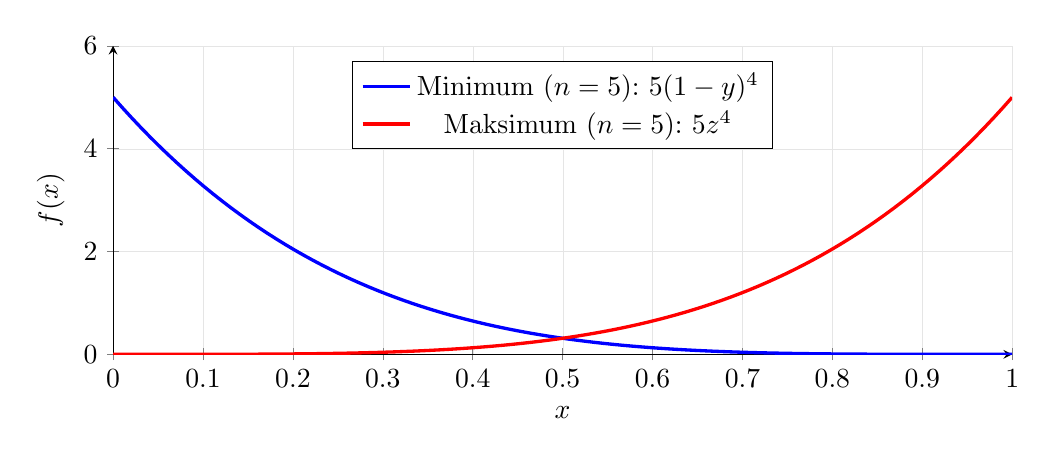
\begin{tikzpicture}
\begin{axis}[
    width=13cm, height=5.5cm,
    axis lines=left,
    xlabel={$x$}, ylabel={$f(x)$},
    xmin=0, xmax=1, ymin=0, ymax=6,
    samples=100, domain=0:1,
    legend style={at={(0.5,0.95)},anchor=north},
    grid=both, grid style={line width=.1pt, draw=gray!20}
]
    \addplot[blue, very thick] {5 * (1 - x)^4};
    \addlegendentry{Minimum ($n=5$): $5(1-y)^4$}

    \addplot[red, very thick] {5 * x^4};
    \addlegendentry{Maksimum ($n=5$): $5z^4$}
\end{axis}
\end{tikzpicture}
\captionof{figure}{$n=5$ için Uniform(0,1) uç değerlerinin yoğunlukları. $n$ büyüdükçe minimum $0$'a, maksimum $1$'e doğru sıkışır.}
\end{center}

\vspace{0.5em}
\section{3. Hafta Ödevi ve Eksiksiz Çözümü}

\begin{odev}{Ki-Kare Dağılımının Standart Normale Yakınsaması}
\textbf{Ödev Sorusu (Sayfa 18):} $Z_n \sim \chi^2_n$ olsun. Standardize edilmiş değişkenin:
\begin{equation}
    Y_n = \frac{Z_n - n}{\sqrt{2n}} \xrightarrow{d} N(0, 1)
\end{equation}
olduğunu gösteriniz. *(Notlarda bu sorunun çözümü boş bırakılmıştır).*

\bigskip
\textbf{1. Çözüm Yolu (Moment Çıkaran Fonksiyon ve Taylor Açılımı):}
$Z_n \sim \chi^2_n$ dağılımının MÇF'si: $M_{Z_n}(t) = (1 - 2t)^{-n/2}$.  
$Y_n = \frac{Z_n - n}{\sqrt{2n}}$ için MÇF'yi kuralım:
\begin{equation}
    M_{Y_n}(t) = e^{-t \sqrt{\frac{n}{2}}} M_{Z_n}\left( \frac{t}{\sqrt{2n}} \right) = e^{-t \sqrt{\frac{n}{2}}} \left( 1 - t \sqrt{\frac{2}{n}} \right)^{-n/2}
\end{equation}
Her iki tarafın doğal logaritmasını alalım:
\begin{equation}
    \ln M_{Y_n}(t) = -t \sqrt{\frac{n}{2}} - \frac{n}{2} \ln\left( 1 - t \sqrt{\frac{2}{n}} \right)
\end{equation}
$\ln(1 - u) = -u - \frac{u^2}{2} - \dots$ Taylor açılımını $u = t \sqrt{\frac{2}{n}}$ için uygulayalım:
\begin{align}
    \ln M_{Y_n}(t) &= -t \sqrt{\frac{n}{2}} - \frac{n}{2} \left[ -t \sqrt{\frac{2}{n}} - \frac{t^2}{n} - O(n^{-3/2}) \right] \notag \\
    &= -t \sqrt{\frac{n}{2}} + t \sqrt{\frac{n}{2}} + \frac{t^2}{2} + O(n^{-1/2}) = \frac{t^2}{2} + O(n^{-1/2})
\end{align}
$n \to \infty$ limitinde:
\begin{equation}
    \lim_{n \to \infty} \ln M_{Y_n}(t) = \frac{t^2}{2} \implies \lim_{n \to \infty} M_{Y_n}(t) = \exp\left( \frac{t^2}{2} \right)
\end{equation}
Bu ifade $N(0, 1)$ dağılımının MÇF'sidir. Dolayısıyla:
\begin{equation}
    \boxed{Y_n = \frac{Z_n - n}{\sqrt{2n}} \xrightarrow{d} N(0, 1)}
\end{equation}

\bigskip
\textbf{2. Çözüm Yolu (CLT Yardımıyla Tek Satırda Çözüm):}
$n$ serbestlik dereceli ki-kare değişkeni, $n$ adet bağımsız $W_i \sim \chi^2_1$ değişkeninin toplamıdır:
\begin{equation}
    Z_n = \sum_{i=1}^n W_i, \quad E(W_i) = 1, \quad V(W_i) = 2
\end{equation}
Merkezi Limit Teoremi gereğince:
\begin{equation}
    \frac{\sum W_i - n E(W_1)}{\sqrt{n V(W_1)}} = \frac{Z_n - n \cdot 1}{\sqrt{n \cdot 2}} = \boxed{\frac{Z_n - n}{\sqrt{2n}} \xrightarrow{d} N(0, 1)}
\end{equation}
\end{odev}

\begin{center}
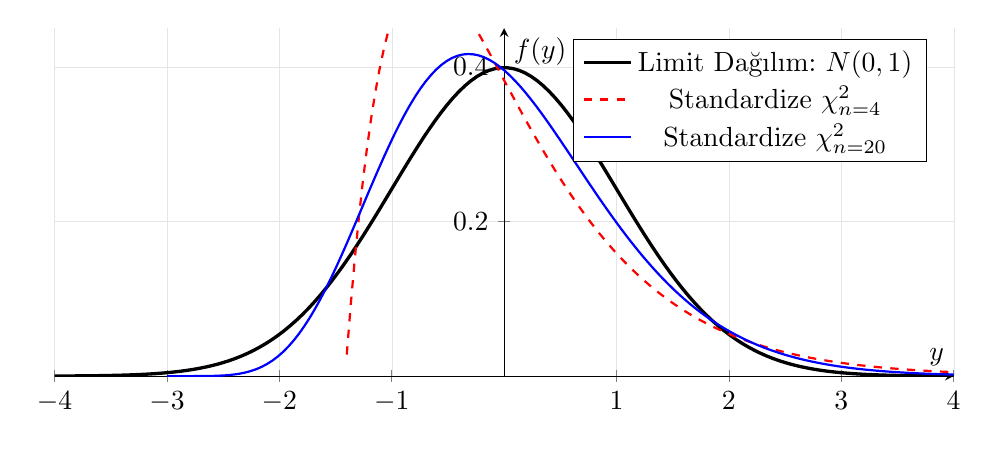
\begin{tikzpicture}
\begin{axis}[
    width=13cm, height=6cm,
    axis lines=center,
    xlabel={$y$}, ylabel={$f(y)$},
    xmin=-4, xmax=4, ymin=0, ymax=0.45,
    samples=150, domain=-4:4,
    legend pos=north east,
    grid=both, grid style={line width=.1pt, draw=gray!20}
]
    \addplot[black, very thick] {1/sqrt(2*pi) * exp(-x^2/2)};
    \addlegendentry{Limit Dağılım: $N(0, 1)$}

    \addplot[red, thick, dashed, domain=-1.4:4] {
        (x*sqrt(8)+4 > 0) * (sqrt(8) * (1/4) * (x*sqrt(8)+4) * exp(-(x*sqrt(8)+4)/2))
    };
    \addlegendentry{Standardize $\chi^2_{n=4}$}

    \addplot[blue, thick, domain=-3:4] {
        (x*sqrt(40)+20 > 0) * (sqrt(40) * (1/(2^10 * 362880)) * (x*sqrt(40)+20)^9 * exp(-(x*sqrt(40)+20)/2))
    };
    \addlegendentry{Standardize $\chi^2_{n=20}$}
\end{axis}
\end{tikzpicture}
\captionof{figure}{Standardize ki-kare değişkenlerinin serbestlik derecesi ($n=4 \to n=20$) arttıkça $N(0,1)$ çan eğrisine kusursuz şekilde yakınsaması.}
\end{center}

\vspace{0.5em}
\section{3. Hafta Hızlı Tekrar ve Yakınsama Türleri Tablosu}

\begin{table}[ht]
\centering
\small
\renewcommand{\arraystretch}{1.35}
\begin{tabularx}{\textwidth}{@{}l l X l@{}}
\toprule
\textbf{Yakınsama Türü} & \textbf{Sembol} & \textbf{Matematiksel Kriter / Anlamı} & \textbf{Güç / Hiyerarşi} \\ \midrule
\textbf{Hemen Hemen H.Y.} & $X_n \xrightarrow{a.s.} X$ & $P(\lim X_n = X) = 1$ (İstisnalar kümesinin olasılığı sıfırdır) & En Güçlü ($\implies P$) \\
\textbf{Momentlerde ($L^r$)} & $X_n \xrightarrow{L^r} X$ & $\lim E(|X_n - X|^r) = 0$ ($r=2$ Ortalama Karede Yakınsama) & Güçlü ($\implies P$) \\
\textbf{Olasılıkta Yakınsama} & $X_n \xrightarrow{P} X$ & $\forall \epsilon > 0, \lim P(|X_n - X| \ge \epsilon) = 0$ (Hedefte sıkışma) & Orta ($\implies d$) \\
\textbf{Dağılımda Yakınsama} & $X_n \xrightarrow{d} X$ & $\lim F_n(x) = F(x)$ veya $\lim M_{X_n}(t) = M_X(t)$ (Şekilce yakınsama) & En Zayıf \\ \bottomrule
\end{tabularx}
\caption{3. Haftada İncelenen 4 Farklı Yakınsama Türünün Özeti ve Hiyerarşik Karşılaştırması}
\end{table}

\end{document}
